\label{subseq:final-results}


Figures \ref{fig:mumps-final-comparison-1} and \ref{fig:mumps-final-comparison-2} show a comparison of MUMPS parallel performance before and after application of above mentioned tuning to GRS matrix set. In case of experiments labeled as \textit{default}, we used ParMetis as a fill reducing reordering algorithm because it had been used by GRS engineers before the current study.\\


\figpointer{\ref{fig:mumps-final-comparison-1}}
\begin{figure}[h!]
\centering
	\begin{tabular}{cc}
		\subfloat[small system: cube-5]{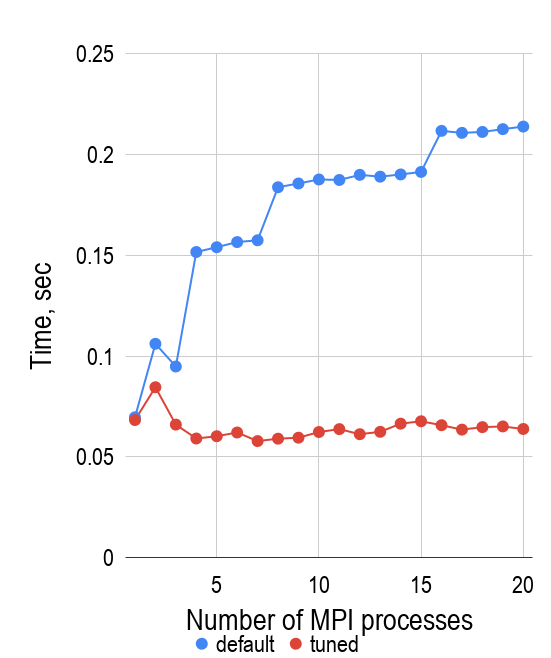
\includegraphics[width=0.43\textwidth]{figures/chapter-2/final-comparison/cube-5.png}} &
		\subfloat[small system: pwr-3d]{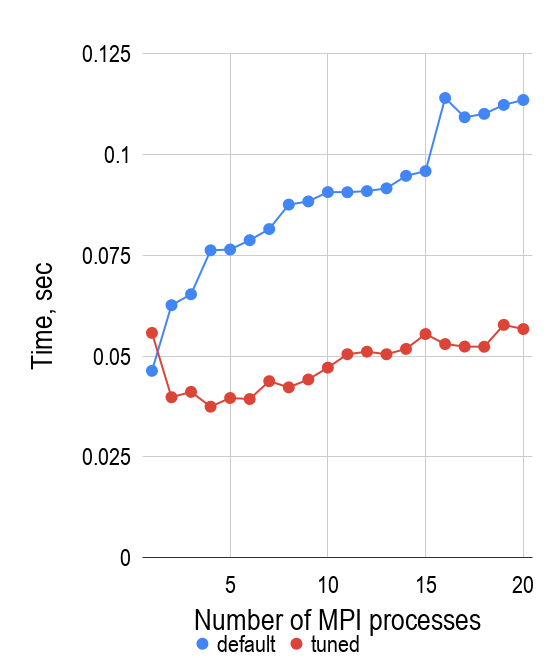
\includegraphics[width=0.43\textwidth]{figures/chapter-2/final-comparison/pwr-3d.png}} \\
	\end{tabular}
	\caption{MUMPS: comparison of different BLAS libraries with using both GRS and SuiteSparse matrix sets on HW1 machine}
	\label{fig:mumps-final-comparison-1}
\end{figure}



\figpointer{\ref{fig:mumps-final-comparison-2}}
\begin{figure}
\centering
	\begin{tabular}{cc}
		\subfloat[medium system: cube-64]{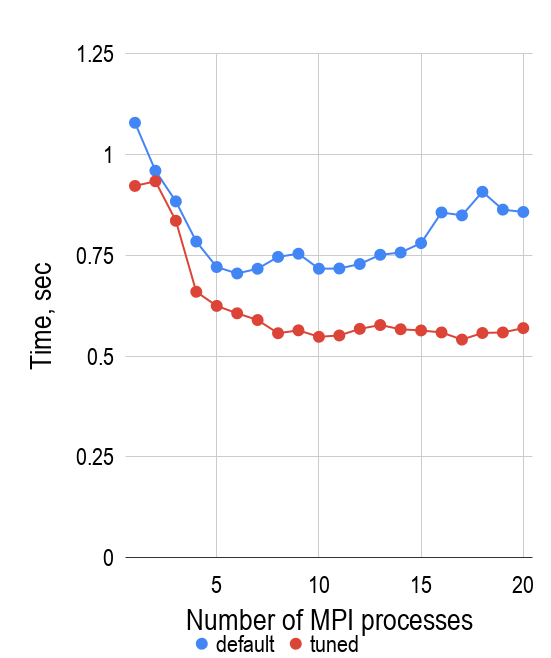
\includegraphics[width=0.48\textwidth]{figures/chapter-2/final-comparison/cube-64.png}} & 			        \subfloat[medium system: k3-2]{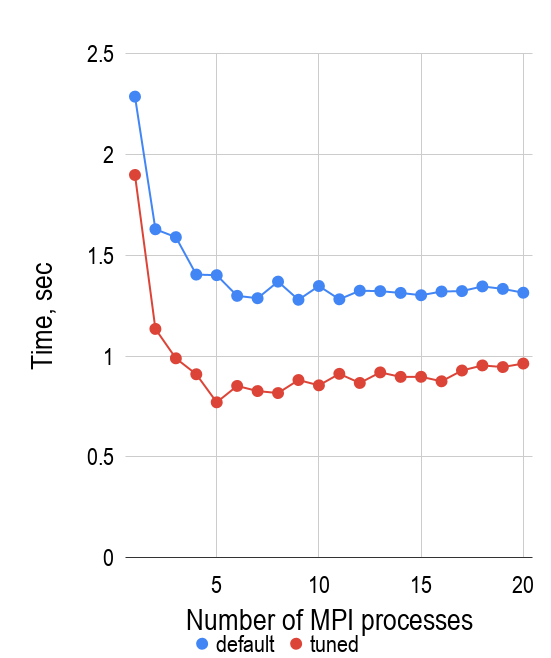
\includegraphics[width=0.48\textwidth]{figures/chapter-2/final-comparison/k3-2.png}} \\
		\subfloat[large system: cube-645\label{fig:mumps-final-comparison-cube-645}]{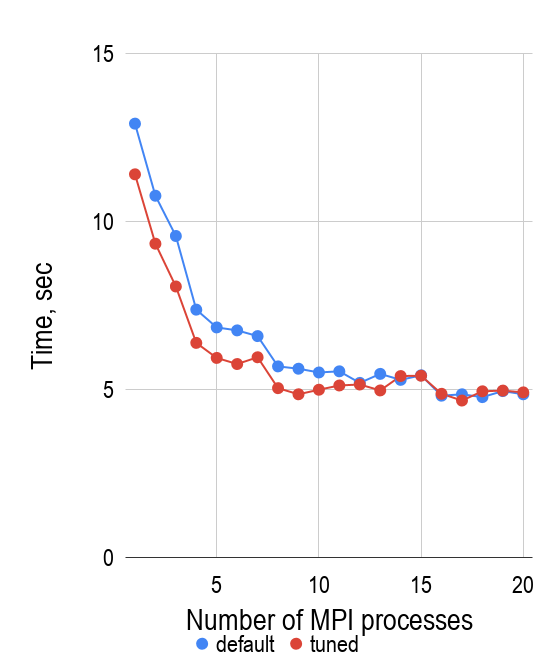
\includegraphics[width=0.48\textwidth]{figures/chapter-2/final-comparison/cube-645.png}} & 			        \subfloat[large system: k3-18\label{fig:mumps-final-comparison-k3-18}]{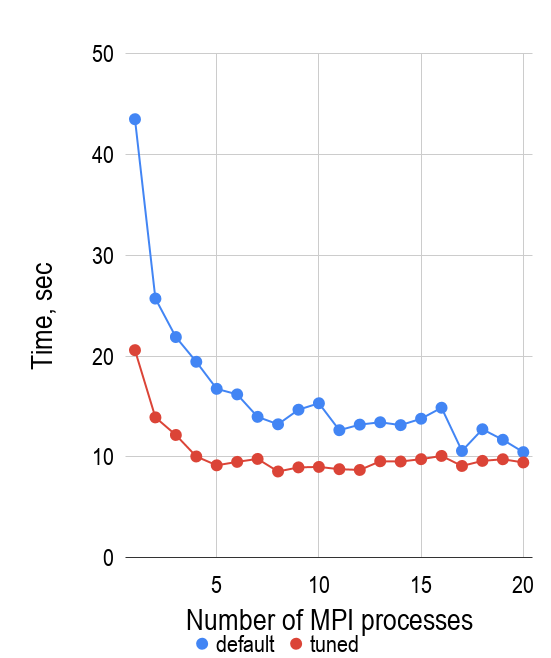
\includegraphics[width=0.48\textwidth]{figures/chapter-2/final-comparison/k3-18.png}} \\
	\end{tabular}
	\caption{MUMPS: comparison of different BLAS libraries with using both GRS and SuiteSparse matrix sets on HW1 machine}
	\label{fig:mumps-final-comparison-2}
\end{figure}

\newpage


\todo{include statistics}
By and large, we have observed significant improvement of applied tuning techniques, mentioned above, for the entire GRS matrix set. \\


In average, the factorization time has been reduced in \textbf{51.4\%} for small sized systems. The significant performance gain mainly came from the optimal choice of fill-in reduction algorithm. Moreover, application of PT-Scotch for small sized systems allowed to drastically change strong scaling behavior and reduce the execution time by approximately \textbf{17\%} in contrast to sequential execution of the default MUMPS configuration that was a challenge before the study.\\


% medium sized systems
The execution time spent on factorization of medium sized systems dropped in \textbf{1.4} times. Additionally, we have noticed that scaling of \textit{cube-64} test case has been considerably changed as it happened in case of small sized systems. Application of PT-Scotch, to \textit{cube-64}, allowed to shift the saturation point from 5 to 10 process count without significant drop of parallel efficiency. All in all, tuning of MUMPS made it possible to reduce the execution time around the saturation points in almost \textbf{31\%} in average for medium sized GRS systems of equations.\\


% larged sized sized system
The factorization performance gain of large sized systems manly came from configuration of MUMPS with optimized BLAS library, OpenBLAS, and MPI \textit{spread} process distribution because it turned out that ParMetis was the best fill-in reduction algorithm for large systems. A noticeable performance gain difference was observed between \textit{cube-645} and \textit{k3-18} test cases. In average, run-time of MUMPS-OpenBLAS configuration reduced by almost \textbf{20\%} in contrast to the default installation in case of \textit{k3-18} whereas factorization time of \textit{cube-645} was improved only by 
\textbf{1.3\%}. However, the saturation points of both cases were shifted towards lower values of the process count which allows to considerably improve hardware utilization  together with improvement of library performance. For example, a detailed study of \textit{k3-18} performance graph, figure \ref{fig:mumps-final-comparison-k3-18}, shows that the saturation point has been moved from 17 to 8 process count. At the same time, the execution time drops by almost \textbf{19\%} and parallel efficiency jumped in about \textbf{13\%}. The same but less significant results can be observed for \textit{cube-645} test case, figure \ref{fig:mumps-final-comparison-cube-645}. \\



%average
% shit of saturation point
% usage of less amount of processing units helps to improve efficiency of the system
% example of k-18, k3-2
% recomendations for small, medium and big GRS systems
